\documentclass{beamer}
\beamertemplatenavigationsymbolsempty
\usepackage{graphicx}
\usepackage{listings}
\lstset{
    breaklines=true,
    numbers=left,
    numberstyle=\scriptsize,
    frame=leftline,
    basicstyle=\ttfamily}

% TODO
%  * use \begin{frame}[fragile] with code examples


\begin{document}
\Large
\begin{frame}

    {\Huge Merged Mining}\\
    \vspace{7mm}
    {\LARGE Ondrej Sika \lstinline|<ondrej@ondrejsika.com>|}\\
    \vspace{7mm}
    {\Large Slush Pool (\url{mining.bitcoin.cz})}\\

\end{frame}

\begin{frame}

    {\Huge Bitcoin}\\

\end{frame}

\begin{frame}

    {\Huge Namecoin}\\

\end{frame}

\begin{frame}

    {\Huge How Bitcoin Mining Works?}\\

\end{frame}

\begin{frame}

    {\Huge Block}\\

    \vspace{5mm}

    * header\\
    * transactions\\


\end{frame}

\begin{frame}

    {\Huge Block Header}\\

    \vspace{5mm}

    * version\\
    * hashPrevBlock\\
    * hashMerkelRoot\\
    * time\\
    * bits (difficulty)\\
    * nonce\\

\end{frame}

\begin{frame}

    {\Huge Blockchain}\\

    \vspace{5mm}

    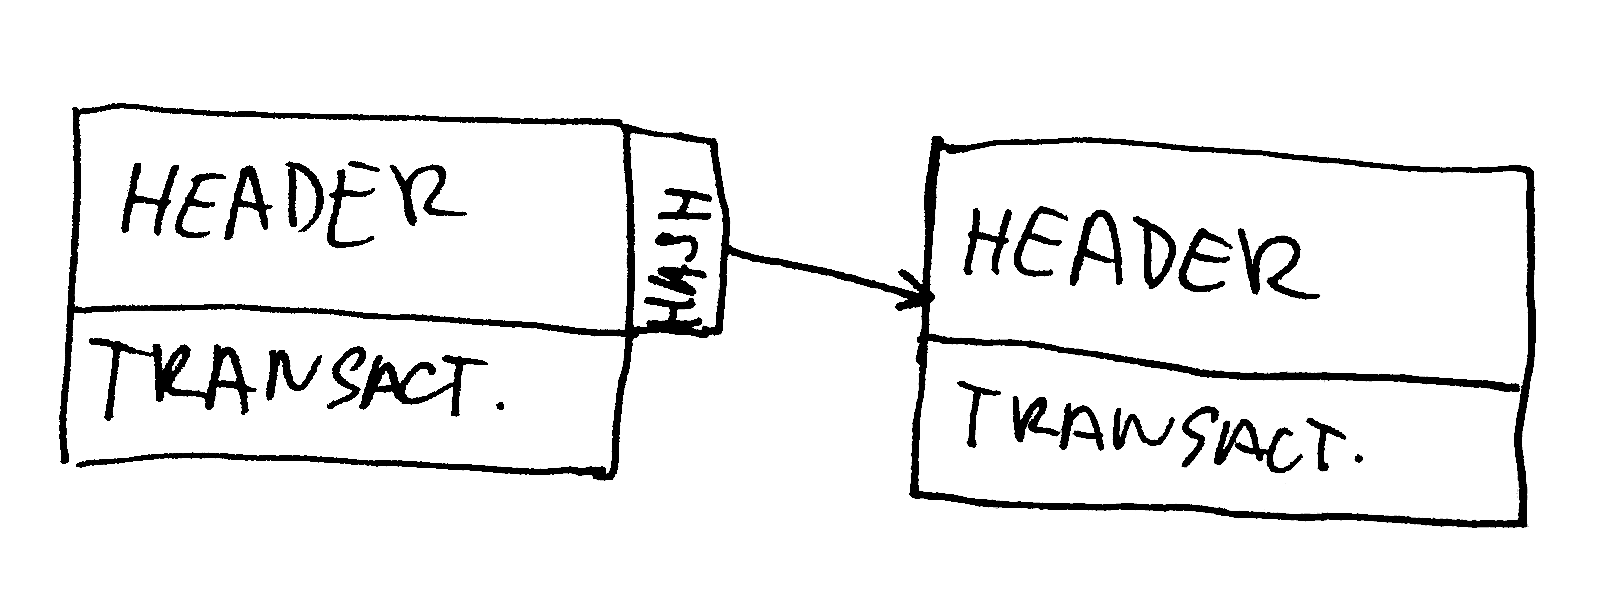
\includegraphics[scale=0.185]{img/blockchain}

\end{frame}

\begin{frame}

    {\Huge Mining}\\

\end{frame}

\begin{frame}

    {\Huge Proof of Work}\\

    \vspace{5mm}

    "A proof of work is a piece of data which was difficult (costly, time-consuming) to produce so as to satisfy certain requirements"\\

\end{frame}

\begin{frame}

    {\Huge Auxiliary POW}\\

    \vspace{5mm}

    "This is the way that merged mining can exist; it is the relationship between two blockchains for one to trust the other's work as their own and accept AuxPOW blocks."\\

\end{frame}

\begin{frame}

    {\Huge Bitcoin Coinbase}\\

    \vspace{5mm}

    * block height\\
    * flags\\
    * merged mining prefix\\
    * namecoin prevhash\\
    * ...\\

\end{frame}

\begin{frame}

    {\Huge Principle of Aux POW}\\

\end{frame}

\begin{frame}

    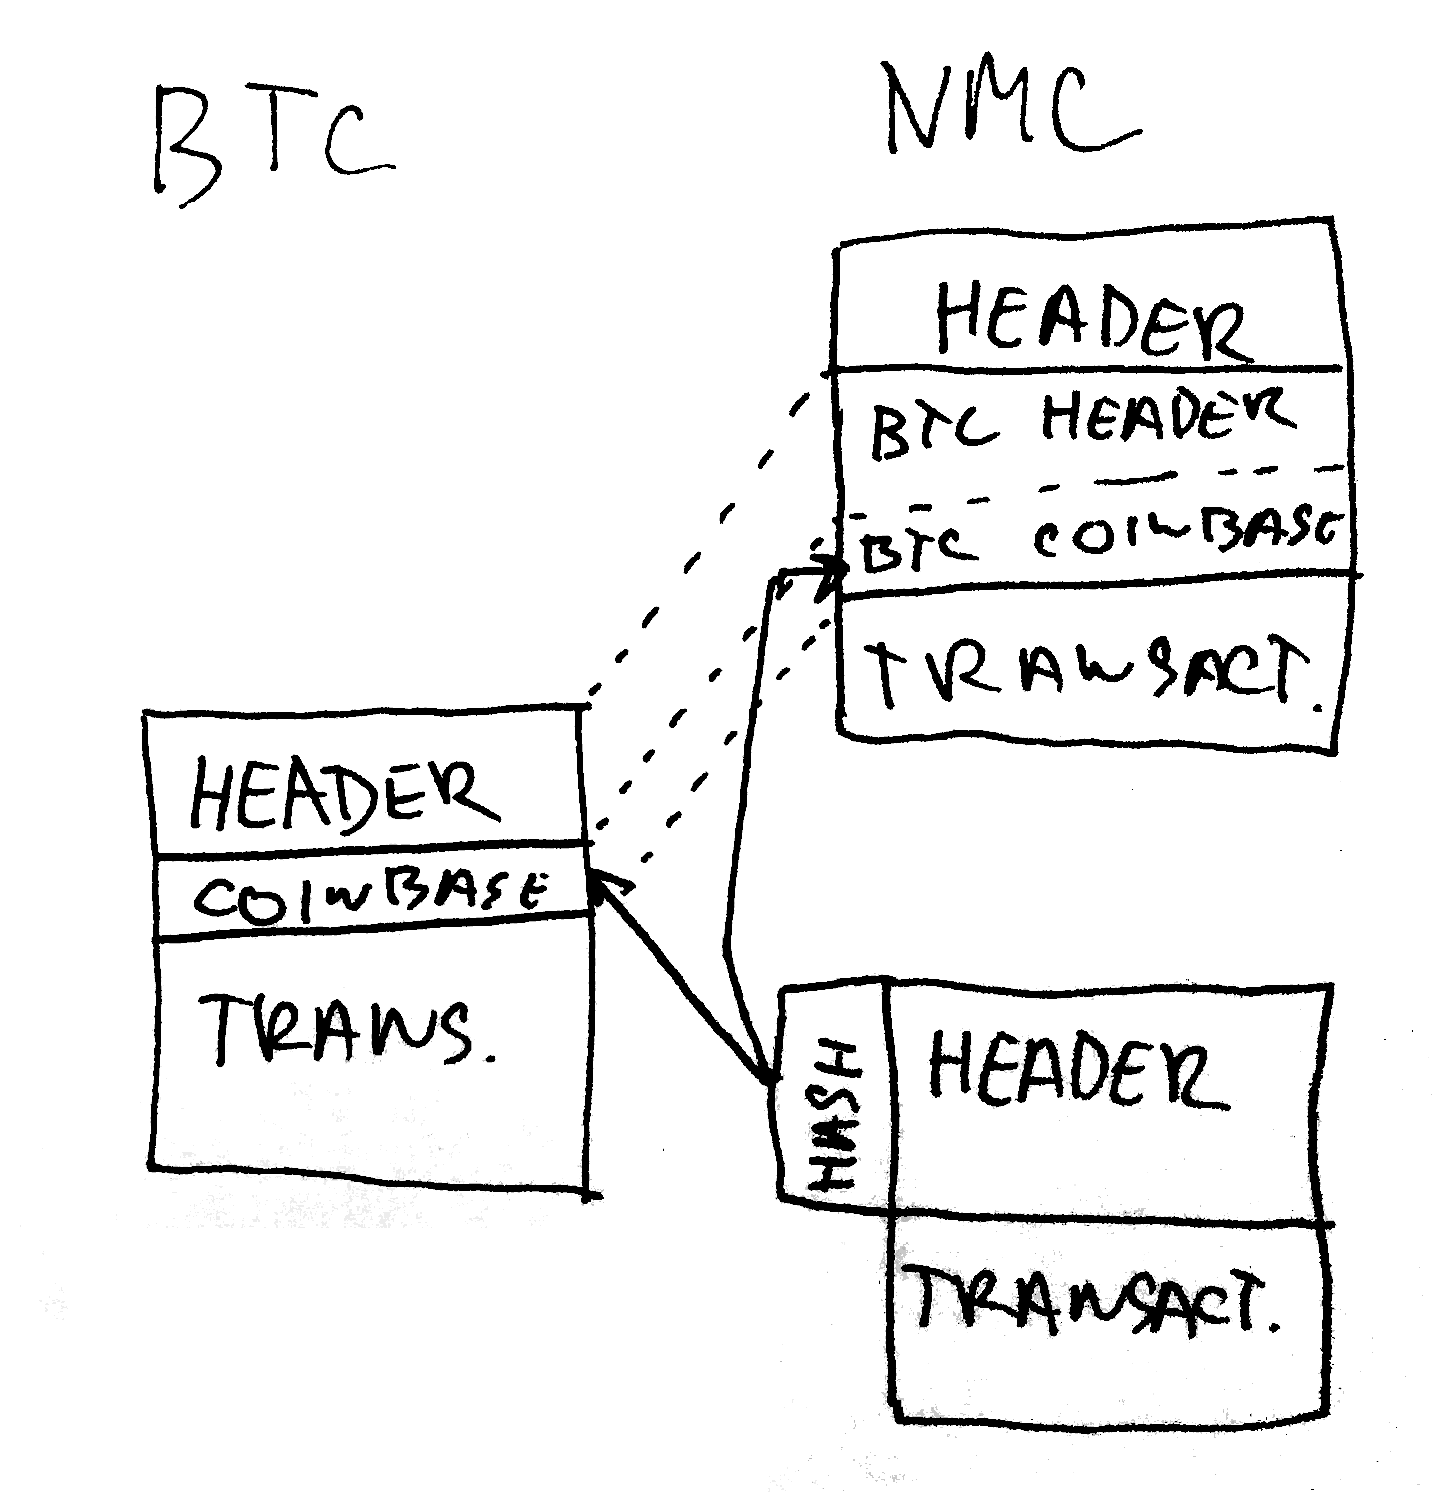
\includegraphics[scale=0.185]{img/principle_of_auxpow}

\end{frame}

\begin{frame}

    {\Huge Namecoin Block}\\

    \vspace{5mm}

    * header\\
    * auxpow (btc coinbase tx, btc branch, btc header)\\
    * transactions\\

%    \vspace{5mm}

%    \begin{tabular}{|l|}
%    \hline
%    HEADER\\
%    \hline
%    BITCOIN BLOCK HEADER\\
%    \hline
%    BITCOIN COINBASE \\
%    \hline
%    TRANSACTIONS\\
%    \hline
%    \end{tabular}

\end{frame}


\begin{frame}

    {\Huge Thanks \& Questions}\\

    \vspace{1cm}

    \texttt{ondrej@ondrejsika.com}\\
    \url{http://ondrejsika.com}\\
    \texttt{@ondrejsika}\\

    \vspace{1cm}

    Sources:\\
    \url{http://url.os1.cz/merged-mining-ctjb/}
\end{frame}

\end{document}

